\documentclass[10pt,french]{article}

\input preambule_2013

\makeatletter
\newcommand\make@car@active[1]{%
	\catcode`#1\active
	\begingroup
		\lccode`\~`#1\relax
		\lowercase{%
	\endgroup\def~}}

\newif\if@shownumline
\newif\if@compil
\newcount\code@line
\newcommand*\shownumline{\@shownumlinetrue}
\newcommand*\hidenumline{\@shownumlinefalse}
\hidenumline

\newcommand\showcode{\@ifstar{\@compilfalse\showcode@i}{\@compiltrue\showcode@i}}

\newcommand\showcode@i{%
	\begingroup
	\parskip\z@\parindent\z@
	\code@line\z@
	\@makeother\;\@makeother\!\@makeother\?\@makeother\:%
	\showcode@}

\newcommand\showcode@[2][50]{%
	\medbreak\noindent
	\begingroup
		\let\do\@makeother\dospecials
		\make@car@active\ { {}}%
		\make@car@active\^^M{\par\leavevmode}%
		\make@car@active\,{\leavevmode\kern\z@\string,}%
		\make@car@active\-{\leavevmode\kern\z@\string-}%
		\showcode@@{#1}{#2}}

\newcommand\showcode@@[3]{%
	\def\@tempa##1#3{\showcode@@@{#1}{#2}{##1}}%
	\@tempa}

\newcommand\showcode@@@[3]{%
	\xdef\the@code{#3}%
	\endgroup
		\vskip0.5ex
		\boxput*(0,1)
			{\fboxsep\z@
			\hbox{\colorbox{black}{\leavevmode\kern0.25em{\bfseries\color{white}\footnotesize\strut#2}\kern0.25em}}%
			}%
			{\fboxsep5pt
			\fbox{%
				$\vcenter{\hsize\dimexpr
					\if@compil0.#1\linewidth-\fboxsep-\fboxrule
					\else\linewidth-2\fboxsep-2\fboxrule\fi\relax
					\kern5pt\parskip0pt \ttfamily\footnotesize
					\begingroup
						\if@shownumline\everypar{\num@code}\fi
						\the@code\par
					\endgroup}%
				\if@compil\vcenter{\kern5pt\hsize\dimexpr\linewidth-0.#1\linewidth-\fboxsep-\fboxrule\relax
					\footnotesize\newlinechar`\^^M\everyeof{\noexpand}\scantokens{#3}}%
				\fi$%
				}%
			}%
	\medbreak
	\endgroup}

\newcommand*\num@code{\hb@xt@4pt{\hss\global\advance\code@line\@ne\tiny\number\code@line}\kern3.5pt }
\makeatother

\PrerenderUnicode{à} % Nécessaire pour les exemples avec accents.

\begin{document}
    
\shownumline % pour numéroter les lignes du code. Pour cacher les numéros : \hidenumline

%-------------------------------------------------------------------------------------------------------
% Structure de la commande \showcode :
% \showcode[< pourcentage de la ligne occupée par le code >]{Titre du code}| < le code ... > |
% la barre verticale | est obtenue avec AltGr + 6
% le retour à la ligne dans le code de gauche n'est pas hyper efficace, il faut donc soi même
% organisé convenablement le code pour ne pas avoir des superpositions comme dans l'exemple 2
%-------------------------------------------------------------------------------------------------------

% ci-dessous, le code occupera 60% de la ligne. 50% est la valeur par défaut.

\showcode[60]{Somme de vecteurs}|
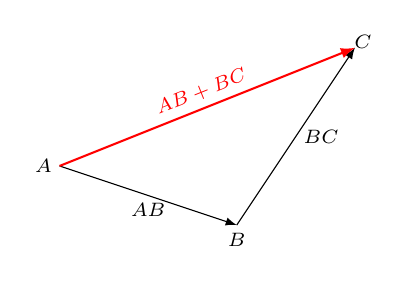
\begin{tikzpicture}[scale=0.75,>=latex]
    \scriptsize
    
    \draw[->] (0,0) node[left] {$A$} -- 
            (3,-1) node[below] {$B$}
            node[midway,below] {$\vect{AB}$};
            
    \draw[->] (3,-1) -- (5,2)
            node[above right=-3pt] {$C$}
            node[midway,right] {$\vect{BC}$};
            
    \draw[->,red,line width=0.75pt] (0,0) -- (5,2)
            node[midway,above,sloped] {$\vect{AB}+\vect{BC}$};
\end{tikzpicture}|

\showcode[50]{Exemple 2}|
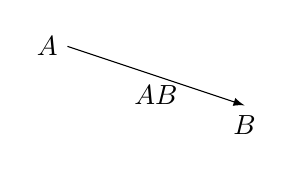
\begin{tikzpicture}[scale=0.75,>=latex]
    \draw[->] (0,0) node[left] {$A$} -- (3,-1) node[below] {$B$} node[midway,below] {$\vect{AB}$};
\end{tikzpicture}|

\hidenumline

\showcode{Exemple avec des accents}|
Il a commandé à boire.
Où doit-il se rendre pour être sûr d'apaiser
sa gorge sèche ?|

%Et voici la version étoilée de la commande \showcode

\showcode*{Exemple non compilé}|
Il a commandé à boire.
Où doit-il se rendre pour être sûr d'apaiser
sa gorge sèche ?|

\end{document}